\documentclass{article}
\usepackage{graphicx} % Required for inserting images
\usepackage{amsmath}
\usepackage[english, russian] {babel}
\usepackage[utf8]{inputenc}
\usepackage[T2A]{fontenc}
\usepackage{minted}
\usepackage{float}
\usepackage{amssymb}

\title{АСА лекция}
\author{silvia.lesnaia }
\date{February 2025}

\begin{document}

\maketitle

\text{11.02.25}

\section{Введение в теорию алгоритмов}

\section{Примеры интуитивного понятия алгоритма}

Алгоритм - точный набор инструкция, описывающих порядок действий исполнителя для достижения результата решения задачи за конечное время

Алгоритм - это понятные и точные предписания исполнителю совершить конченное число шагов, направленных на решение поставленной задачи

Алгоритм - это конеченый набор правил, который определяет последовательность операций


\subsection{Основные свойства алгоритмов}

Дискретность

Детерминированность

Понятность

Завершаеомсть

Массовость

Однозначность результата 



\subsection{Основные задачи теории алгоритмов}

формализация понятия «алгоритм» и  исследование формальных алгоритмических систем;

формальное доказательство алгоритмической неразрешимости ряда задач;

классификация задач, определение и исследование сложностных классов;

асимптотический анализ сложности алгоритмов;

исследование и анализ рекурсивных алгоритмов;

получение явных функций трудоемкости в целях сравнительного анализа алгоритмов;

разработка критериев сравнительной оценки качества алгоритмов.

\subsection{Схема определения понятия «алгоритм»:}

Понятие данных

Память

Элементарный шаг

Детерминированность

Результативность

\subsection{Основные типы алгоритмических моделей}
Алгоритм как некое детерминированное устройство - абстрактные машины. 
Машина Тьюринга и машина Поста.

Алгоритм как процедура вычисления некой числовой функции. Рекурсивные функции Черча.

Алгоритм как последовательность преобразований цепочек в каком-либо алфавите.
(Комбинаторные операции над словами). Нормальные алгоритмы Маркова.

\section{Машина Поста}

Тезис Поста - “Всякий алгоритм представим в форме машины Поста”.

Алгоритм (по Посту) — программа для машины Поста, приводящая к решению поставленной задачи.

Если задача имеет алгоритмическое решение, то она представима в форме команд для машины Поста.


\begin{figure}
    \centering
    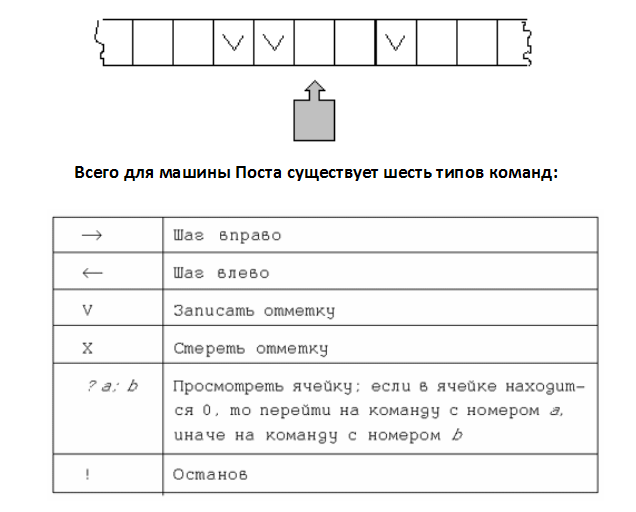
\includegraphics[width=1\linewidth]{Снимок экрана 2025-02-25 090545.png}
\end{figure}


\subsection{Варианты окончания выполнения программы на машине Поста}

останов по команде "стоп". 
Такой останов называется результативным и указывает на корректность алгоритма;

останов при выполнении недопустимой команды. 
Случаи, когда указатель должен записать метку там, где она уже есть, 
или стереть метку там, где ее нет;

машина не останавливается никогда. Уход в бесконечность, зацикливание.


\subsection{Примеры}

Пример: покажем, как можно воспользоваться командой условного перехода 
для организации циклического процесса. 
Пусть на ленте имеется запись из нескольких меток подряд, 
и головка находится над самой крайней меткой справа. 
Требуется перевести головку влево до первой пустой позиции.

			$1\leftarrow 2$

			$2 ? 3; 1$

			$3 !$


 Пример: увеличить число 3 на единицу (изменить значение в памяти с 3 на 4). 
 Допустим, точно известно, что каретка стоит где-то слева от меток и обозревает пустую ячейку. 
 Тогда программа увеличения числа на единицу может выглядеть так:

 1 -> 2

 2 ? 1;3

 3 <- 4

 4 V 5

 5 !
 


Пример: на ленте машины Поста расположен массив из n меток. 
Составить программу, действуя по которой машина выяснит, делится ли число n на 3. 
Если да, то после массива через одну пустую ячейку поставить метку.

$1 \rightarrow 2 $

$2 ? 3;4$

$3 !$

$4 \rightarrow 5$

$5 ? 3;6$

$6 \rightarrow 7$

$7 \& 8;1$

$8 \rightarrow 9$

$9 V 3$

Пример: зацикливание. 

$1 → 2$

$2 ← 1$


6 вариант 
\begin{figure}
    \centering
    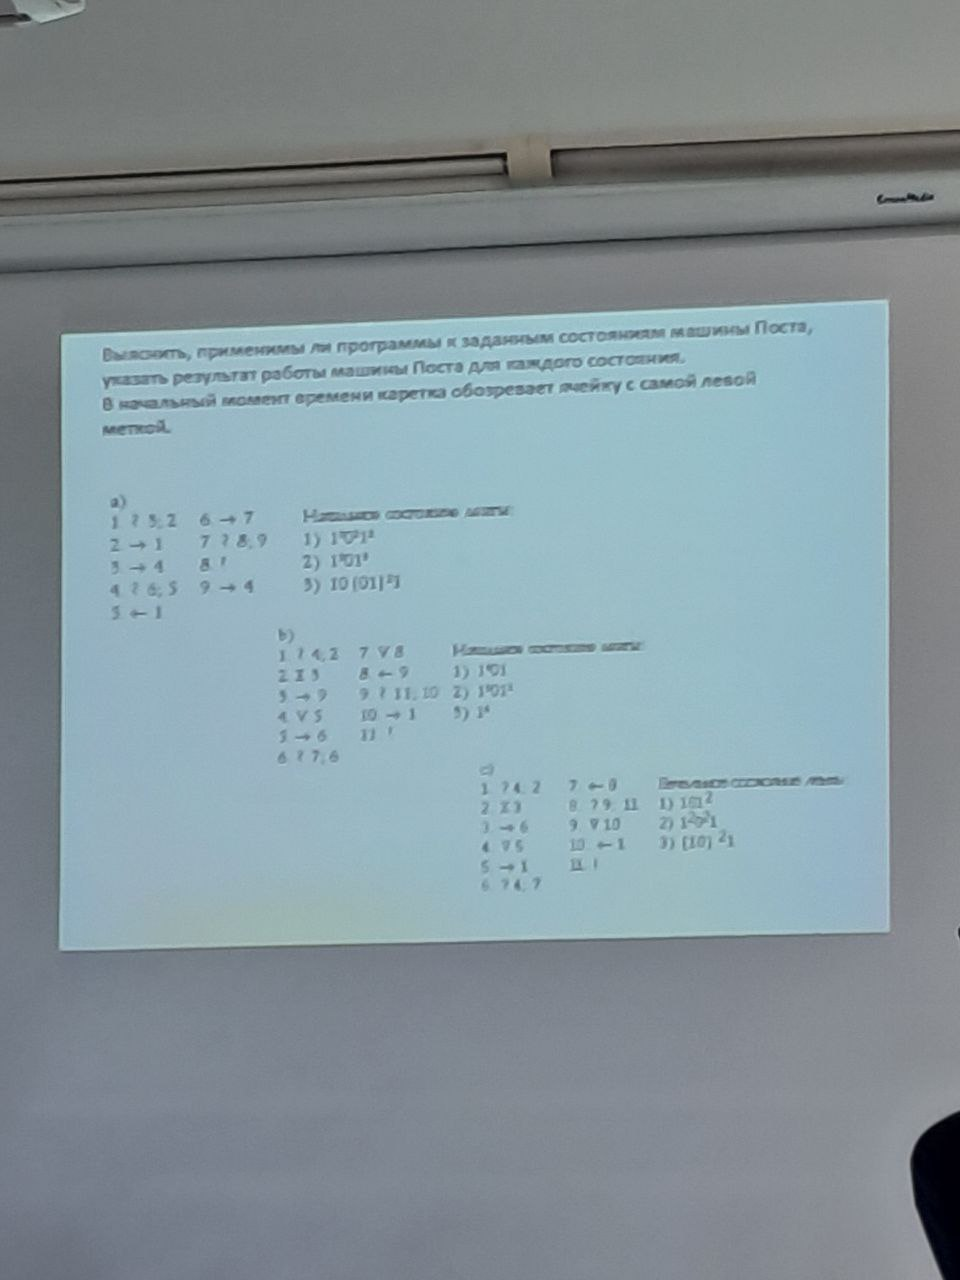
\includegraphics[width=1\linewidth]{photo_5285451810783490009_y.jpg}

Ответ: 01010110
    
\end{figure}

\vspace{10mm}

\textbf{18.02.25}

\section{Машина Тюрингита}

\subsection{Формальное описание машины Тюрингита}

\subsection{Способы задания МТ}

    Граф переходов

    \subsection{Конфигурация МТ}

    Совокупность состояний ленты, указаний на ленте

    Протоколы - 

    \subsection{Приведений конфигураций к стандартному виду}

    \subsection{Определение вычислимости по Тьюрингу}




\vspace{10mm}

\textbf{25.02.25}

\section{Приницип суперпозиции}

\section{Оператор примитивной рекурисии}


окончание перовй презентации тезис Черча

начало второй презентации

\section{Алгоритм Маркова}



\section{Алгоритмически неразрешимые задачи}


\section{Основы задачи ... }


\textbf{25.03.25}

\section{NP}
Задачи, которые нельзя отнести ни к классу P, ни к классу E.

Задачи, которые недетерминированная машина Тьюринга может решить
 за полиномиальное время, тогда как для детерминированной машины Тьюринга
  полиномиальный алгоритм неизвестен.

Для этих задач до сих пор не разработан эффективный
 (т.е. полиномиальный) алгоритм, но и не доказано,
  что таких алгоритмов не существует.

К классу NP относятся все задачи, решение которых можно проверить 
за полиномиальное время. 
Оракул предлагает решения, которые после проверки верификатором 
за полиномиальное время приобретают «юридическую» силу.

\textbf{Пример}

Дано n чисел $a_1,…a_n$ и число V.

Задача: Найти вектор (массив) X=($x_1,…,x_n$), $x_i\in{0,1}$, такой, что $\sum a_ix_i = V$.
Т.е. может ли быть представлено число V в виде
 суммы каких- либо элементов массива А.

Если какой-то алгоритм выдает результат – массив
 X, то проверка правильности этого результата може
 т быть выполнена с полиномиальной сложностью: проверка

$\sum a_ix_i = V$ требует не более $\circleddash $ (N) операций.

\subsection{Проблема равенсства классов P и NP}


Поскольку детерминированная машина Тьюринга может рассматриваться
 как специальный случай недетерминированной машины Тьюринга,
  в которой отсутствует стадия угадывания, 
  а стадия проверки совпадает с ДМТ, класс NP включает в себя класс P,
   а также некоторые проблемы, для решения которых известны лишь алгоритмы, 
   экспоненциально зависящие от размера входа 
   (то есть неэффективные для больших входов).

Вопрос о равенстве этих двух классов
 считается одной из самых сложных открытых проблем
  в области теоретической информатики.

  \begin{figure} [H]
    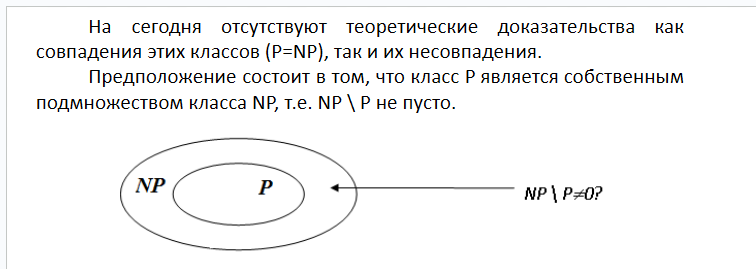
\includegraphics[width=1\linewidth]{Снимок экрана 2025-03-25 093755.png}
\end{figure}

  \subsection{Класс NPC (NP – полные задачи)}

  Определение класса NPC (NP-complete) или класса NP-полных задач
   требует выполнения следующих двух условий: во-первых,
    задача должна принадлежать классу NP, и, во-вторых,
     к ней полиномиально должны сводиться все задачи из класса NP

     \begin{figure} [H]
        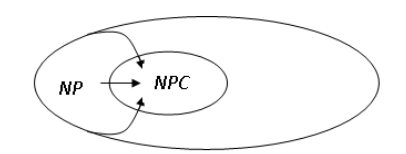
\includegraphics[width=0.50\linewidth]{Снимок экрана 2025-03-25 093930.png}
    \end{figure}


    \text{Полиномиальная сводимость}

    Сведение по Карпу

    ....

    Свудение по Куку

....

    Для класса NPC доказана следующая теорема:
     если существует задача, принадлежащая классу NPC,
      для которой существует полиномиальный алгоритм решения, то класс P совпадает с классом NP, т.е. P=NP
	В настоящее время доказано существование сотен NP– полных задач,
     но ни для одной из них пока не удалось найти полиномиального алгоритма решения.
      В настоящее время исследователи предполагают следующее соотношение классов:

      тут должна быть кортинка


\textbf{01.04.25}



\section{Вычисление времени выполнения нерекурсивных алгоритмов}
\subsection{Нахождение функции трудоемкости по фактическому количеству элементарных операций}


В качестве «элементарных» операций алгоритма, представленного 
в формальной системе RAM будем использовать следующие:
1) простое присваивание: а $\leftarrow$ b;
2) одномерная индексация a[i];
3) арифметические операции: (*, /, -, +);
4) операции сравнения;
5) логические операции. 


\textbf{Анализ трудоемкости основных алгоритмических конструкций}

\begin{figure} [H]
    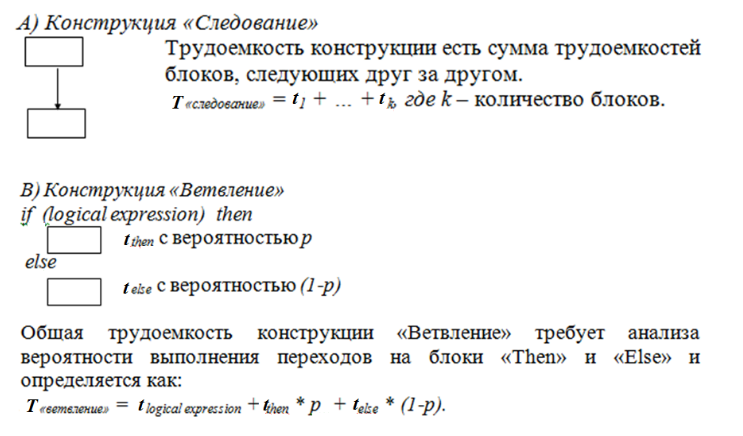
\includegraphics[width=1\linewidth]{Снимок экрана 2025-04-01 090309.png}
\end{figure}



\vspace{1cm}

\textbf{15.04.25}


метод рекрентных соотношений

\end{document}